% This is compiled and printed on the back of the board!
% NOTE TO SELF: Dice faces use the LaTeX font that starts with j iirc

\documentclass{article}
\pagenumbering{gobble}

\usepackage[papersize={10in,10in},margin=0.3in]{geometry}
\usepackage{fontspec}
\usepackage{multicol}
\usepackage{graphicx}
\usepackage{titlesec}

\setmainfont{GFS Didot}
\newfontfamily\Racing{Faster One}

\titleformat{\section}[runin]{%
    \fontsize{16}{16}\Racing}{}{0em}{}
\titlespacing*{\section}{0pt}{0pt}{1em}

\begin{document}
\begin{multicols}{3}

\section{Setup}

    \textsc{To} begin the game separate out the upgrade cards from the rest of the cards.
    You should be left with the starter cards (grey border), and the stretch
    cards (have a distance at the bottom).

    Separate the starter cards into 4 equal decks (with the exact same cards in
    them).

    Setup the rest of the game by giving each player a starting deck, a red die,
    a blue die, and a token. Their token should be placed before the starting
    line on the map.

\section{Objective}

    \textsc{This} is a race. Just like the real iditarod your goal is to be the first to
    travel 1600km (160 myriameters). Each square on the board is a single
    myriameter, so there are 160 of them.

\section{Costs}

    \textsc{The} core mechanic of this game is the way in which costs on cards are
    played.

    When a card is played the three costs are resolved in order.

    First, the player must discard a number of cards equal to the "energy" cost
    (blue number) of the card from their hand.

    Second, the player must discard a number of cards equal to the "health" cost
    (red number) of the card from the top of their deck. If the player fails to
    pay either cost, the card does nothing.

    Finally the player must resolve the "risk" of the card.

\section{Risk}

    \textsc{Whatever} the risk (black number) of a card is, that many cards must be
    played from the top of your deck on the subsequent turns successfully. Only
    once all such cards are played does the effect of the original card take
    place.

    If another risk occurs as payment for a risk they do stack, but once the
    risk of the second card is paid its effect happens even if the original risk
    card's effect has not.

    If at any point you cannot afford the cards being played as risk, the risk
    card fizzles and does nothing.

\section{New Days}

    \textsc{On} any turn a player may choose to take a new day instead of playing a card.
    In this case any current risk the player is in the process of resolving are
    abandoned and the player shuffles their discard pile and hand into their
    deck and draw a new starting hand.

    At this point any of the other players may choose to partake in the new day,
    taking the same actions as the player who initiated it, or race through the
    night and continue as they are.

    Additionally some cards and stretches have effects that occur at the
    beginning or end of a day. A day is marked by whenever any player causes a
    new day, not just the player to whom the effect applies.

    The starting hand is, by default, 6 cards. This number is frequently
    modified however.

\section{Weather}

    \textsc{At} the start of each new day, roll the white weather die to determine the
    weather for the day. The effects are as follows:

    \begin{itemize}
        \setlength\itemsep{-1em}
        \item 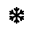
\includegraphics[width=1.5em]{images/die/snowflake} Snowy weather cancels all sled cards.
        \item 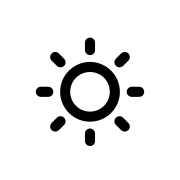
\includegraphics[width=1.5em]{images/die/sun} Sunny weather provides a +1 speed bonus.
        \item 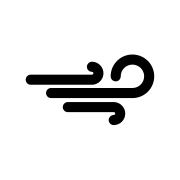
\includegraphics[width=1.5em]{images/die/wind} Windy weather provides a +5 speed bonus but gives all players hypothermia.
        \item 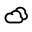
\includegraphics[width=1.5em]{images/die/cloud} Cloudy weather gives a -1 speed penalty.
        \item 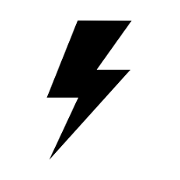
\includegraphics[width=1.5em]{images/die/storm} Stormy weather cancels all movement.
        \item 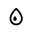
\includegraphics[width=1.5em]{images/die/rain} Rainy weather provides a +3 speed bonus but gives all players starvation.
    \end{itemize}

\section{Destruction}

    \textsc{There} is an important distinction between discarding and destroying a card.
    When a card is discarded it is merely added to its player's discard pile and
    will return to their deck when they take a new day. A card which is
    destroyed is removed from play and will not be used in the current game ever
    again.

\section{Stretch Effects}

    \textsc{Each} stretch has a unique effect when you enter it. Like other cards,
    stretches may have red and blue numbers on them. These set your starvation
    and hypothermia respectively.

    Starvation increases the health (red) cost of every card by 1 for each
    starvation you have. This does not apply to cards with no health cost to
    begin with. Keep track of starvation on your sled card using the red die.

    Hypothermia increases the energy (blue) cost of every card by 1 for each
    hypothermia you have. This does not apply to cards with no energy cost to
    begin with. Keep track of hypothermia on your sled card using the blue die.

    If either your starvation or hypothermia reaches a level of 6 you have died.
    Move back 30 myriameters and set your starvation and hypothermia to that of
    your current track. If you move beyond the town you will have 0 starvation
    and hypothermia.

\section{Special Effects}

    \textsc{Recover} allows you to move the specified number of cards from your discard
    pile into either your hand or your deck. The choice is yours.

    When you pass a player on the board you take 1 damage and they are moved
    back 1 square. This process occurs iteratively, so there can never be two
    players on the same space of the board (except before the starting line).
    The direction of movement does not matter, if you become further ahead of
    someone you take a damage and they move back one, even if they were moving
    backwards.

\section{Card Types}

    \textsc{The} following is a summary of how each card type works:

    \begin{itemize}
        \setlength\itemsep{-0.8ex}
        \item \textsc{Dog} cards are brown. When you play a dog it stays in front of you
            and provides a passive bonus. You may only have 6 dogs at a time,
            but may kill a dog whenever you wish. A killed dog is destroyed (not
            discarded).

        \item \textsc{Attachment} cards are blue. You must play an attachment on a dog
            and dogs may only hold one attachment each. You may not remove an
            attachment once played. Like dogs, attachments provide passive
            bonuses. When the dog an attachment is on is killed, that attachment
            is discarded.

        \item \textsc{Food} cards are yellow. As soon as you play a food card your
            starvation is reduced by 1. This happens before payment and whether
            or not payment succeeds.

        \item \textsc{Personal} cards are purple. As soon as you play a personal card
            your hypothermia is reduced by 1. This happens before payment and
            whether or not payment succeeds. Personal cards typically have the
            text "Destroy up to X of Y" on them. This means that you look at the
            top Y cards of your deck, choose up to X of them to destroy, then
            choose which of the remaining cards to shuffle back into your deck
            and which to draw into your hand. Using a personal card is referred
            to as "healing".

        \item \textsc{Sled} cards are green. They typically have the text "Take X of Y"
            on them. This means that you look at the top Y cards of the upgrade
            deck, choose X of them to place in your discard pile, and destroy
            the rest. As they are immediately discarded all other players may
            see what they are. Additionally you may not use them until the next
            day (unless you recover them).

        \item \textsc{Utility} cards are white. They tend to be interactive. They have no
            effect whatsoever when you are immune. This means that they do
            nothing if you play them, and do not effect you if someone else
            plays them. Remove the utility cards from the game when playing
            solitaire.

        \item \textsc{Movement} cards are blue. When you play a movement card add your
            current speed to its effect.
    \end{itemize}

\end{multicols}
\end{document}
